\section{Captain}

\begin{minipage}{0.5\textwidth}
\textbf{Function}: Chief of the guards, rules his subjects and runs the jail

\subsubsection{Internal World}

\textbf{Age \& Gender}: 40, Male \\
\textbf{Values \& Virtues}: Loyal to the queen\\
\textbf{Ethnic Group}: Human/Demon

\subsection{External World}
\textbf{Environment}: Castle of Dynamia \\
\textbf{Look \& Feel}: Tall, big and fat man\\
\textbf{Type of attack}: Melee and ranged \\
\end{minipage}%
%
\hfill\begin{minipage}{0.4\textwidth}
  \begin{figure}[H]
  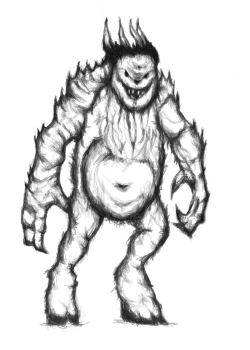
\includegraphics{Images/Enemies/captain_portrait}
   \caption{Sketch of the captain made by Elena Coperchini}
  \end{figure}
\end{minipage}

\subsubsection{Description and background story}
The captain was, without any doubt, the strongest and scariest man who ever joined the guards and, due to this, Mizar has chosen him for one of her experiments. Given his extreme faith, loyalty and submission to the queen, the captain immediately accepted her offer and so Mizar blended him with one of her demons making him even stronger, scarier and faster. He is the boss of the level "In the enemy territory" and attack any intruder as soon as he sees them.

\subsection{Finite State Machine}
\begin{figure}[H]
  \centering
  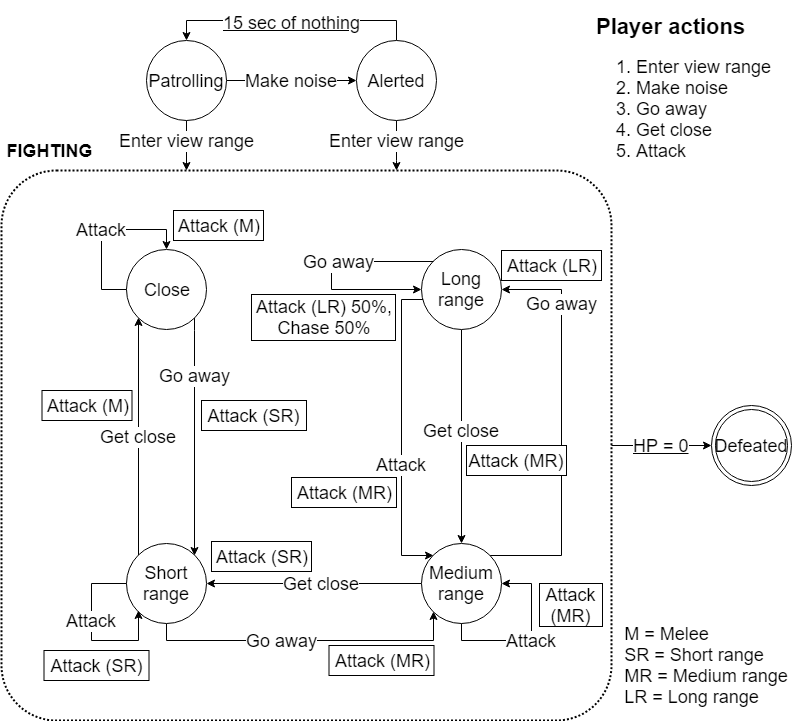
\includegraphics[width=\textwidth]{Images/Diagrams/FSMs/captainFSM}
  \caption{FSM for the captain}
\end{figure}

\begin{itemize}
	\item \textbf{Patrolling}: the captain roams around in its area and looks around.
	\item \textbf{Alerted}: the captain moves towards the noise source and looks around for the player.
	\item \textbf{Fighting}: when entering in Fighting mode, the captain transforms in half demon.
	\begin{itemize}
		\item \textbf{Close}: the captain attacks the player (melee attack).
		\item \textbf{Short range}: the captain attacks the player (short range attack).
		\item \textbf{Medium range}: the captain attacks the player (medium range attack).
		\item \textbf{Long range}: the captain moves towards the player.
	\end{itemize}
	\item \textbf{Defeated}: the half demon transformation ends and the captain falls down confused.
\end{itemize}

The captain has two attacks: Magic claw and Fireball.

The Magic claw is a melee attack that scratches Sophie. It is a more powerful version of the demons' Claw attack. When attacking, the claws of his right hand glow with purple light and leave a trial of the same color that stands for a second.

The Fireball is a ranged attack. The captain creates a fireball between his hands and then he throws it with his right hand against the target.

For more reference images: \url{http://wastelandsteam.altervista.org/captain/}\\
Password: \textit{gld18}
